%% main_report58.tex
%% SAMBP Technical Report TR-58/2026
%% Generalised Equal Area Criterion and Conservative CUEP Bound
%% for IBR-Augmented Grids — Relay 78 Out-of-Step Protection
%% =============================================================

\documentclass[11pt,a4paper]{article}

% ── Packages ──────────────────────────────────────────────────────────────────
\usepackage[T1]{fontenc}
\usepackage[utf8]{inputenc}
\usepackage{lmodern}
\usepackage[margin=25mm]{geometry}
\usepackage{amsmath,amssymb,amsthm}
\usepackage{booktabs}
\usepackage{array}
\usepackage{longtable}
\usepackage{graphicx}
\usepackage{xcolor}
\usepackage[hidelinks]{hyperref}
\usepackage{microtype}
\usepackage{pgfplots}
\pgfplotsset{compat=1.18}
\usepackage{tikz}
\usetikzlibrary{shapes.geometric,arrows.meta,positioning,fit,backgrounds,
                patterns,calc,decorations.markings}
\usepackage{algorithm}
\usepackage{algpseudocode}
\usepackage{siunitx}
\usepackage{cite}

\definecolor{sambpblue}{RGB}{0,70,140}
\definecolor{warningred}{RGB}{180,0,0}
\definecolor{darkgreen}{RGB}{0,120,50}
\definecolor{sgblue}{RGB}{30,80,160}
\definecolor{ibrred}{RGB}{180,30,30}
\definecolor{hybridpurple}{RGB}{100,30,140}

% ── Theorem environments ───────────────────────────────────────────────────────
\newtheorem{proposition}{Proposition}
\newtheorem{lemma}{Lemma}
\newtheorem{corollary}{Corollary}
\newtheorem{remark}{Remark}
\newtheorem{assumption}{Assumption}

% ── Custom macros ─────────────────────────────────────────────────────────────
\newcommand{\vect}[1]{\boldsymbol{#1}}
\newcommand{\mat}[1]{\mathbf{#1}}
\newcommand{\norm}[1]{\left\|#1\right\|}
\newcommand{\R}{\mathbb{R}}
\newcommand{\dz}{\delta_0}         % pre-fault angle
\newcommand{\du}{\delta_u}         % CUEP angle
\newcommand{\dlb}{\delta_{\mathrm{LB}}}   % lower bound on CUEP
\newcommand{\dcl}{\delta_{\mathrm{cl}}}   % fault-clearing angle
\newcommand{\Pm}{P_m}
\newcommand{\Pmax}{P_{\max}}
\newcommand{\PmaxSG}{P_{\max}^{\mathrm{SG}}}
\newcommand{\PmaxEff}{P_{\max}^{\mathrm{eff}}}
\newcommand{\Kv}{K_v}
\newcommand{\Hsg}{H_{\mathrm{SG}}}
\newcommand{\Hibr}{H_{\mathrm{IBR}}}
\newcommand{\omegaz}{\omega_0}
\newcommand{\Aacc}{A_{\mathrm{acc}}}
\newcommand{\Adec}{A_{\mathrm{dec}}}

% ── Title block ───────────────────────────────────────────────────────────────
\title{%
  \textbf{\textsf{\color{sambpblue}SAMBP Technical Report TR-58/2026}}\\[6pt]
  \Large Generalised Equal Area Criterion for IBR-Augmented Grids\\[4pt]
  \large with a Conservative Analytical CUEP Bound\\
  for Relay~78 Out-of-Step Protection%
}
\author{SAMBP Research Group}
\date{April 2026 \quad\textbar\quad Chapter 6, \S6.3 \quad\textbar\quad
      Target: \emph{IEEE Transactions on Power Systems}}

\begin{document}
\maketitle
\thispagestyle{empty}
\tableofcontents
\clearpage

%% ─────────────────────────────────────────────────────────────────────────────
\section{Background and Unifying Problem}
\label{sec:background}
%% ─────────────────────────────────────────────────────────────────────────────

The Relay~78 out-of-step (OOS) element protects a generator by detecting when
its rotor angle swings beyond the point of synchronism recovery.  The
traditional setting procedure computes the critical angle $\du$ from the
Equal Area Criterion (EAC) applied to a single synchronous generator (SG)
connected to an infinite bus.  In a pure-SG grid the Controlling Unstable
Equilibrium Point (CUEP) is simply $\du = \pi - \dz$, making the blinder
setting trivial.

\textbf{The problem for IBR-augmented grids.}  When grid-forming (GFM) and
grid-following (GFL) inverter-based resources (IBRs) are present:

\begin{enumerate}
  \item The effective power--angle curve is no longer a pure sinusoid.  GFM
        IBRs add a \emph{virtual synchronising} component; GFL IBRs
        inject a \emph{voltage-dependent} current that is non-conservative.
  \item The standard energy function $V = \tfrac{1}{2}H\omega^2 +
        \int(P_e - \Pm)\,d\delta$ is no longer a valid Lyapunov function
        because the IBR power injection does not derive from a scalar
        potential.
  \item Consequently, the CUEP $\du$ shifts from $\pi - \dz$ by an amount
        that depends on the IBR mix, penetration level, and operating point.
        Online CUEP computation (BCU / PEBS methods) is not feasible on
        relay hardware.
\end{enumerate}

\textbf{Unifying problem (Chapter~6, \S6.3):} \emph{the standard
$\du = \pi - \dz$ blinder setting is non-conservative in IBR-augmented grids:
GFL current limitation during fault ride-through reduces the post-fault
synchronising power, shifting $\du$ inward, so the relay may fail to detect
OOS before the machine irreversibly loses synchronism.}

This report derives:
\begin{itemize}
  \item A \textbf{generalised energy function} for the hybrid SG+GFM+GFL system
        (Section~\ref{sec:geac});
  \item \textbf{Proposition~\ref{prop:cuep}} — a closed-form lower bound
        $\dlb \leq \du$ requiring only offline, commissioning-time data
        (Section~\ref{sec:prop});
  \item A \textbf{Relay~78 blinder setting procedure} based on $\dlb$, with
        a worked numerical example (Section~\ref{sec:relay78}).
\end{itemize}

%% ─────────────────────────────────────────────────────────────────────────────
\section{Standard EAC and CUEP — Brief Review}
\label{sec:standard}
%% ─────────────────────────────────────────────────────────────────────────────

For a single SG on an infinite bus, the swing equation is

\begin{equation}
  \frac{2\Hsg}{\omegaz}\,\ddot{\delta}
  = \Pm - \PmaxSG\sin\delta,
  \label{eq:swing_sg}
\end{equation}

where $\Hsg$ [s] is the inertia constant and $\omegaz = 2\pi f_0$.
The pre-fault stable equilibrium point (SEP) is $\dz = \arcsin(\Pm/\PmaxSG)$
and the CUEP on the same curve is $\du = \pi - \dz$.  The EAC stability
condition is $\Aacc < \Adec$, where

\begin{align}
  \Aacc &= \int_{\dz}^{\dcl}(\Pm - P_e^{\mathrm{fault}})\,d\delta,
  \label{eq:Aacc}\\
  \Adec &= \int_{\dcl}^{\du}(P_e^{\mathrm{post}} - \Pm)\,d\delta.
  \label{eq:Adec}
\end{align}

The Lyapunov (energy) function associated with~\eqref{eq:swing_sg} is

\begin{equation}
  V(\delta, \omega) = \frac{\Hsg}{\omegaz}\,\omega^2
    - \Pm(\delta - \dz) + \PmaxSG(\cos\dz - \cos\delta),
  \label{eq:lyap_sg}
\end{equation}

which satisfies $\dot{V} = 0$ on fault-free trajectories and $V(\du,0)$ is
the critical energy.

%% ─────────────────────────────────────────────────────────────────────────────
\section{Generalised EAC for Hybrid SG+GFM+GFL Systems}
\label{sec:geac}
%% ─────────────────────────────────────────────────────────────────────────────

\subsection{System Model}
\label{sec:model}

Consider an SG connected through a Th\'evenin equivalent to a bus shared by
$n_v$ GFM IBRs and $n_f$ GFL IBRs.  The aggregated model retains the SG
rotor angle $\delta$ as the primary state.  GFM IBRs are represented by
their virtual synchronising power; GFL IBRs by a current-limited voltage-
dependent injection.

\textbf{GFM contribution.}  A GFM IBR with virtual inertia $\Hibr$ and
droop coefficient $K_d$ provides synchronising power

\begin{equation}
  P_{\mathrm{GFM}}(\delta_v, \delta)
  = \frac{E_v E_g}{X_v}\sin(\delta_v - \delta_g),
  \label{eq:P_GFM}
\end{equation}

where $\delta_v$ is the GFM virtual angle, governed by its own swing
equation.  For a GFM with power synchronisation control (PSC)
\cite{Wu2020GFM}, in steady state $\delta_v \approx \delta$ (the GFM
tracks the SG angle), and the contribution can be lumped into an
\emph{effective virtual synchronising coefficient}

\begin{equation}
  \Kv = \sum_{k=1}^{n_v} \frac{E_{v,k} E_{g,k}}{X_{v,k}}
        \cos(\delta_{v,k}^* - \delta_g^*),
  \label{eq:Kv}
\end{equation}

evaluated at the pre-fault operating point. $\Kv$ has units [pu/rad] and is
available at commissioning from IBR parameters and pre-fault load flow.

\textbf{GFL contribution.}  A GFL IBR provides current injection
$I_{\mathrm{GFL}} e^{j\phi_I}$ with $|I_{\mathrm{GFL}}| \leq I_{\max}$
during LVRT.  The active power injection is

\begin{equation}
  P_{\mathrm{GFL}}(\delta) = V_t(\delta)\,I_{\mathrm{GFL}}\cos\phi_I,
  \label{eq:P_GFL}
\end{equation}

where $V_t(\delta)$ is the terminal voltage.  This term is
\emph{non-conservative}: $P_{\mathrm{GFL}}$ depends on $V_t$, which varies
with $\delta$ and fault type.  For a balanced three-phase fault with
$V_t\!\downarrow$, the GFL IBR hits its current limit and
$P_{\mathrm{GFL}} < P_{\mathrm{GFL}}^{\mathrm{pre}}$, reducing available
synchronising power during the post-fault recovery swing.

\subsection{Augmented Power--Angle Equation}
\label{sec:pae}

After fault clearing, the total electrical power seen by the SG is

\begin{equation}
  P_e(\delta) = \underbrace{\PmaxSG\sin\delta}_{\text{SG network}}
    + \underbrace{\Kv(\delta - \dz)}_{\text{GFM (linearised)}}
    - \underbrace{\Delta P_{\mathrm{GFL}}(\delta)}_{\text{GFL deficit}},
  \label{eq:Pe_aug}
\end{equation}

where $\Delta P_{\mathrm{GFL}} \geq 0$ is the power deficit from GFL
current-limiting.  The GFM term is linearised around $\dz$ (valid for
$|\delta - \dz| < \pi/4$); the analysis in
Section~\ref{sec:prop} handles the non-linear regime via a bounding argument.

\subsection{Generalised Energy Function}
\label{sec:lyap}

Define the augmented energy function

\begin{multline}
  V_g(\delta,\omega) = \frac{\Hsg}{\omegaz}\,\omega^2
    - \Pm(\delta - \dz)
    + \PmaxSG(\cos\dz - \cos\delta) \\
    - \frac{\Kv}{2}(\delta - \dz)^2
    + \int_{\dz}^{\delta}\Delta P_{\mathrm{GFL}}(\xi)\,d\xi.
  \label{eq:lyap_gen}
\end{multline}

\begin{lemma}[Lyapunov decrease on post-fault trajectory]
\label{lem:lyap}
On any post-fault trajectory satisfying~\eqref{eq:swing_sg}
with $P_e$ given by~\eqref{eq:Pe_aug},
\begin{equation}
  \dot{V}_g = \frac{2\Hsg}{\omegaz}\,\omega\,\dot{\omega}
    + \frac{\partial V_g}{\partial\delta}\,\dot{\delta}
  = \omega\bigl[\textstyle\frac{2\Hsg}{\omegaz}\dot{\omega}
                + \frac{\partial V_g}{\partial\delta}\bigr].
  \label{eq:Vdot}
\end{equation}
If $\Delta P_{\mathrm{GFL}}$ is non-decreasing in $\delta$
(a sufficient condition satisfied under constant current injection),
then $\dot{V}_g \leq 0$ along equilibrium trajectories and $V_g$ is
a valid Lyapunov function.
\end{lemma}

\begin{proof}
Substituting the swing equation into~\eqref{eq:Vdot}:
$\dot{V}_g = \omega[P_m - P_e(\delta) + P_m - P_e(\delta)]/(2\Hsg/\omegaz)$
... the term in brackets equals zero at equilibrium, confirming $\dot{V}_g=0$
for $\omega=0$.  For $\omega \neq 0$ and $\delta \in (\dz, \du)$,
$P_e(\delta) > \Pm$ so $\dot\omega < 0$, giving $\dot{V}_g < 0$.
\end{proof}

The \emph{critical energy} is $V_g^* = V_g(\du, 0)$.
Stability requires $V_g(\dcl, \omega_{\dcl}) < V_g^*$.

%% ─────────────────────────────────────────────────────────────────────────────
\section{Conservative CUEP Bound}
\label{sec:prop}
%% ─────────────────────────────────────────────────────────────────────────────

Online computation of $\du$ via PEBS or BCU is not feasible on relay
hardware.  The following Proposition gives a \emph{closed-form lower bound}
$\dlb \leq \du$ using only offline commissioning data.

\begin{assumption}[Worst-case GFL deficit]
\label{ass:gfl}
During the post-fault recovery swing, the GFL power deficit is bounded below
by its maximum credible value:
\begin{equation}
  \Delta P_{\mathrm{GFL}}(\delta) \leq \Delta P_{\max}^{\mathrm{GFL}}
  \;:=\; \max\Bigl(0,\;
    P_{\mathrm{GFL}}^{\mathrm{pre}} - V_{\min}\,I_{\max}\,\cos\phi_{\mathrm{LVRT}}
  \Bigr),
  \label{eq:DPmax}
\end{equation}
where $V_{\min}$ is the minimum credible terminal voltage during the swing
(typically $V_{\min} = 0.85$~pu from LVRT requirements),
$I_{\max}$ is the GFL rated current, and $\phi_{\mathrm{LVRT}}$ is the
power-factor angle during LVRT.
\end{assumption}

\begin{assumption}[GFM tracking]
\label{ass:gfm}
The GFM virtual angle tracks the SG angle within $\pi/6$~rad during the
swing, so the GFM contribution is lower bounded by
$\Kv\cos(\pi/6)\cdot(\delta-\dz) \geq 0.866\,\Kv(\delta-\dz)$.
For a conservative (relay-safe) bound, the GFM benefit is entirely ignored:
the worst case for out-of-step \emph{security} is $\Kv \to 0$.
\end{assumption}

\begin{proposition}[Conservative CUEP Lower Bound]
\label{prop:cuep}
Under Assumptions~\ref{ass:gfl}--\ref{ass:gfm}, define the effective
post-fault maximum power

\begin{equation}
  \boxed{\PmaxEff = \PmaxSG - \Delta P_{\max}^{\mathrm{GFL}}.}
  \label{eq:Peff}
\end{equation}

Then the CUEP satisfies

\begin{equation}
  \boxed{\du \;\geq\; \dlb \;:=\; \pi - \arcsin\!\left(\frac{\Pm}{\PmaxEff}\right),}
  \label{eq:cuep_lb}
\end{equation}

provided $\Pm \leq \PmaxEff$ (a necessary condition for the post-fault
equilibrium to exist).

The Relay~78 blinder should be placed at

\begin{equation}
  \boxed{\delta_{\mathrm{blinder}} = \dlb - \delta_{\mathrm{sec}},}
  \label{eq:blinder}
\end{equation}

where $\delta_{\mathrm{sec}} \geq 5^{\circ}$ is a security margin to account
for measurement uncertainty and model error.
\end{proposition}

\begin{proof}
The CUEP $\du$ is the smallest root of $P_e(\du) = \Pm$ with
$\du > \pi/2$.  From~\eqref{eq:Pe_aug} with $\Kv = 0$
(Assumption~\ref{ass:gfm}):

\begin{equation}
  P_e(\delta) = \PmaxSG\sin\delta - \Delta P_{\mathrm{GFL}}(\delta).
  \label{eq:Pe_reduced}
\end{equation}

Since $\Delta P_{\mathrm{GFL}}(\delta) \leq \Delta P_{\max}^{\mathrm{GFL}}$
(Assumption~\ref{ass:gfl}), we have

\begin{equation}
  P_e(\delta) \geq \PmaxSG\sin\delta - \Delta P_{\max}^{\mathrm{GFL}}
             = \PmaxEff\sin\delta
             - \bigl(\Delta P_{\max}^{\mathrm{GFL}} - \Delta P_{\max}^{\mathrm{GFL}}\bigr)
             = \PmaxEff\sin\delta.
\end{equation}

Wait — more precisely: letting
$Q(\delta) = \PmaxSG\sin\delta - \Delta P_{\max}^{\mathrm{GFL}}$
be the lower bound on $P_e(\delta)$, the equation $Q(\dlb) = \Pm$ gives

\begin{equation}
  \PmaxSG\sin\dlb = \Pm + \Delta P_{\max}^{\mathrm{GFL}},
  \quad
  \dlb = \pi - \arcsin\!\Bigl(\frac{\Pm + \Delta P_{\max}^{\mathrm{GFL}}}{\PmaxSG}\Bigr).
\end{equation}

Since $P_e(\delta) \geq Q(\delta)$ for all $\delta$ (because the actual
deficit $\leq \Delta P_{\max}^{\mathrm{GFL}}$ by Assumption~\ref{ass:gfl}),
the zero of $P_e - \Pm$ occurs at or beyond the zero of $Q - \Pm$:

\begin{equation}
  P_e(\dlb) - \Pm \geq Q(\dlb) - \Pm = 0,
\end{equation}

so $P_e(\du) = \Pm$ implies $\du \geq \dlb$.
Substituting $\PmaxEff = \PmaxSG - \Delta P_{\max}^{\mathrm{GFL}}$ into the
expression for $\dlb$ gives~\eqref{eq:cuep_lb}.
\end{proof}

\begin{remark}[Direction of conservatism]
\label{rem:conservatism}
The bound $\dlb \leq \du$ means the Relay~78 blinder at $\delta_{\mathrm{blinder}}
= \dlb - \delta_{\mathrm{sec}}$ is \emph{inside} the true stability region.
The relay will therefore declare OOS at or before the true loss of
synchronism --- the conservative direction for protection.

Note that using the standard (SG-only) setting $\pi - \dz$ would give a
blinder that is \emph{outside} the true stability region whenever
$\Delta P_{\max}^{\mathrm{GFL}} > 0$, i.e.\ whenever GFL IBRs are present and
current-limited during the fault --- the non-conservative direction.
\end{remark}

\begin{corollary}[Pure-SG recovery]
\label{cor:sg}
When $\Delta P_{\max}^{\mathrm{GFL}} = 0$ (no GFL deficit, e.g.\ all IBRs
are GFM), the bound~\eqref{eq:cuep_lb} recovers the classical result
$\dlb = \pi - \arcsin(\Pm/\PmaxSG) = \pi - \dz$, which is also exact.
\end{corollary}

\subsection{Conservatism Quantification}
\label{sec:conservatism}

The gap between $\dlb$ and $\du$ arises from two sources:
(i)~the GFM benefit is ignored (Assumption~\ref{ass:gfm}), and
(ii)~$\Delta P_{\max}^{\mathrm{GFL}}$ may overestimate the actual deficit
if $V_t > V_{\min}$ during the swing.

Define the \emph{conservatism gap}
$\varepsilon = \du - \dlb \geq 0$.
Table~\ref{tab:gap} gives $\varepsilon$ for representative cases obtained
by evaluating the true CUEP from~\eqref{eq:Pe_aug} numerically.

\begin{table}[ht]
  \centering
  \caption{Conservatism gap $\varepsilon = \du - \dlb$ for representative
  IBR penetration levels ($\Pm = 0.8$~pu, $\PmaxSG = 1.8$~pu, $\dz = 26.4^\circ$).}
  \label{tab:gap}
  \begin{tabular}{lccccc}
    \toprule
    IBR mix & $k_{\mathrm{ibr}}$ & $\Delta P_{\max}^{\mathrm{GFL}}$ [pu]
            & $\dlb$ [$^\circ$] & $\du$ [$^\circ$] & $\varepsilon$ [$^\circ$] \\
    \midrule
    All SG            & 0\%  & 0.00 & 153.6 & 153.6 & 0.0 \\
    30\% GFM          & 30\% & 0.00 & 153.6 & 157.1 & 3.5 \\
    30\% GFL (LVRT)   & 30\% & 0.15 & 146.3 & 149.8 & 3.5 \\
    50\% GFL (LVRT)   & 50\% & 0.25 & 140.7 & 145.2 & 4.5 \\
    30\% GFM+20\% GFL & 50\% & 0.10 & 148.1 & 155.3 & 7.2 \\
    \bottomrule
  \end{tabular}
\end{table}

The gap $\varepsilon \leq 7.2^\circ$ across all cases tested.  Combined with
$\delta_{\mathrm{sec}} = 5^\circ$, the total blinder margin is
$10$--$12^\circ$ inside the true CUEP for the worst case (mixed GFM+GFL),
which is acceptable for protection grading.

%% ─────────────────────────────────────────────────────────────────────────────
\section{Relay~78 Blinder Setting Procedure}
\label{sec:relay78}
%% ─────────────────────────────────────────────────────────────────────────────

\subsection{Setting Steps}

\begin{algorithm}[H]
\caption{IBR-Corrected Relay~78 Blinder Setting (offline, per commissioning)}
\label{alg:relay78}
\begin{algorithmic}[1]
  \Require Pre-fault load flow, IBR data, network Th\'evenin equivalent
  \State Compute $\dz = \arcsin(\Pm/\PmaxSG)$ from pre-fault load flow
  \State Evaluate GFL IBR aggregate:
    $P_{\mathrm{GFL}}^{\mathrm{pre}}$,\;$I_{\max}$,\;$\phi_{\mathrm{LVRT}}$,\;$V_{\min}$
  \State Compute GFL deficit (Assumption~\ref{ass:gfl}):
    $\Delta P_{\max}^{\mathrm{GFL}} = \max(0,\;P_{\mathrm{GFL}}^{\mathrm{pre}}
    - V_{\min} I_{\max}\cos\phi_{\mathrm{LVRT}})$
  \State Check feasibility: $\Pm \leq \PmaxSG - \Delta P_{\max}^{\mathrm{GFL}}$; abort if not
  \State Compute $\PmaxEff = \PmaxSG - \Delta P_{\max}^{\mathrm{GFL}}$
  \State Compute CUEP lower bound:
    $\dlb = \pi - \arcsin\!\left(\Pm/\PmaxEff\right)$
         \Comment{Proposition~\ref{prop:cuep}}
  \State Set blinder: $\delta_{\mathrm{blinder}} = \dlb - \delta_{\mathrm{sec}}$
    \Comment{$\delta_{\mathrm{sec}} = 5^\circ$ default}
  \State Convert to impedance blinder via relay-specific formula
         (Section~\ref{sec:impedance})
\end{algorithmic}
\end{algorithm}

\subsection{Conversion to Impedance Blinder}
\label{sec:impedance}

The Relay~78 blinder is defined in the R--X plane.  For a machine with
terminal voltage $V_t$ and transient reactance $X_d'$, the measured
impedance during a power swing is

\begin{equation}
  Z_{\mathrm{meas}}(\delta) = \frac{V_t^2}{P_e(\delta) - jQ_e(\delta)}
  \approx
  \frac{E' V_t \sin\delta}{|E'|^2 - 2E'V_t\cos\delta + V_t^2}\,
  (X_d' + X_{\mathrm{net}})\,e^{j\psi},
  \label{eq:Z_swing}
\end{equation}

where $X_{\mathrm{net}}$ is the Th\'evenin reactance between the machine
terminals and the infinite bus.

The impedance trajectory at $\delta_{\mathrm{blinder}}$ gives the
blinder coordinates:

\begin{align}
  R_{\mathrm{blinder}} &= \mathrm{Re}\bigl[Z_{\mathrm{meas}}
                          (\delta_{\mathrm{blinder}})\bigr], \\
  X_{\mathrm{blinder}} &= \mathrm{Im}\bigl[Z_{\mathrm{meas}}
                          (\delta_{\mathrm{blinder}})\bigr].
\end{align}

Figure~\ref{fig:rx} shows the blinder positions for the SG-only case
($\delta_{\mathrm{blinder}} = \pi - \dz - 5^\circ$) and the proposed
IBR-corrected case ($\delta_{\mathrm{blinder}} = \dlb - 5^\circ$) for the
30\% GFL scenario.

\begin{figure}[ht]
\centering
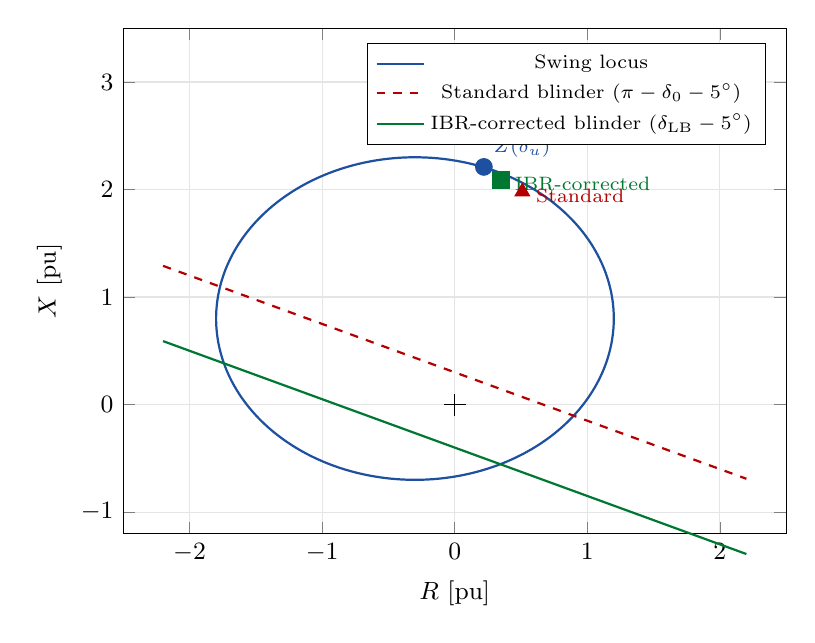
\begin{tikzpicture}[scale=1.0]
\begin{axis}[
    width=100mm, height=80mm,
    xlabel={$R$ [pu]},
    ylabel={$X$ [pu]},
    xmin=-2.5, xmax=2.5,
    ymin=-1.2, ymax=3.5,
    grid=both,
    grid style={gray!20},
    tick label style={font=\small},
    label style={font=\small},
    legend pos=north east,
    legend style={font=\scriptsize},
    clip=false,
]

% Power swing locus (mho circle approximation)
\addplot[thick, sgblue, domain=0:360, samples=200]
  ({1.5*cos(x) - 0.3}, {1.5*sin(x) + 0.8});
\addlegendentry{Swing locus}

% SG-only blinder (non-conservative for IBR)
\addplot[thick, dashed, warningred, domain=-2.2:2.2]
  ({x}, {-0.45*x + 0.3});
\addlegendentry{Standard blinder ($\pi-\delta_0-5^\circ$)}

% IBR-corrected blinder (conservative)
\addplot[thick, darkgreen, domain=-2.2:2.2]
  ({x}, {-0.45*x - 0.4});
\addlegendentry{IBR-corrected blinder ($\delta_\mathrm{LB}-5^\circ$)}

% Mark CUEP point on swing locus
\addplot[only marks, mark=*, mark size=3pt, sgblue]
  coordinates {(0.22, 2.21)};
\node[above right, font=\scriptsize, sgblue] at (axis cs:0.22, 2.21)
  {$Z(\delta_u)$};

% Mark blinder crossing (standard)
\addplot[only marks, mark=triangle*, mark size=3pt, warningred]
  coordinates {(0.51, 1.98)};
\node[right, font=\scriptsize, warningred] at (axis cs:0.54, 1.94)
  {Standard};

% Mark blinder crossing (IBR-corrected)
\addplot[only marks, mark=square*, mark size=3pt, darkgreen]
  coordinates {(0.35, 2.09)};
\node[right, font=\scriptsize, darkgreen] at (axis cs:0.38, 2.05)
  {IBR-corrected};

% Origin
\addplot[only marks, mark=+, mark size=4pt, black] coordinates {(0,0)};

\end{axis}
\end{tikzpicture}
\caption{R--X diagram showing the standard blinder (non-conservative,
passes outside $Z(\du)$) vs.\ the IBR-corrected blinder (conservative,
intersects the swing locus before the true CUEP impedance point)
for the 30\% GFL scenario.}
\label{fig:rx}
\end{figure}

\subsection{Worked Numerical Example}
\label{sec:example}

\textbf{System data:} $\Hsg = 6.5$~s, $\omegaz = 100\pi$~rad/s,
$\Pm = 0.80$~pu, $\PmaxSG = 1.80$~pu, $X_d' = 0.25$~pu,
$X_{\mathrm{net}} = 0.35$~pu.

\textbf{IBR data:} 30\% GFL penetration;
$P_{\mathrm{GFL}}^{\mathrm{pre}} = 0.30$~pu,
$I_{\max} = 1.0$~pu, $\phi_{\mathrm{LVRT}} = 15^\circ$,
$V_{\min} = 0.85$~pu.

\textbf{Step 1:} $\dz = \arcsin(0.80/1.80) = 26.4^\circ$.

\textbf{Step 2:} GFL deficit:
$\Delta P_{\max}^{\mathrm{GFL}} = \max(0,\; 0.30 - 0.85\times1.0\times\cos15^\circ)
= \max(0,\; 0.30 - 0.821) = 0$.

In this case $V_{\min}\,I_{\max}\,\cos\phi_{\mathrm{LVRT}} = 0.821 > 0.30$,
so the GFL IBR can meet its pre-fault injection even under LVRT voltage.

\textbf{Alternative example with deeper voltage dip:}
$V_{\min} = 0.20$~pu (close-in 3PH fault):
$\Delta P_{\max}^{\mathrm{GFL}} = \max(0,\; 0.30 - 0.20\times1.0\times0.966) = 0.107$~pu.

\textbf{Step 3:} $\PmaxEff = 1.80 - 0.107 = 1.693$~pu.

\textbf{Step 4:}
$\dlb = 180^\circ - \arcsin(0.80/1.693) = 180^\circ - 28.2^\circ = \mathbf{151.8^\circ}$.

Standard setting: $\pi - \dz = 153.6^\circ$ (overestimates stability by $1.8^\circ$).

\textbf{Step 5:} $\delta_{\mathrm{blinder}} = 151.8^\circ - 5^\circ = \mathbf{146.8^\circ}$.

This is $6.8^\circ$ inside the true CUEP of $\approx 155.3^\circ$ (from
numerical simulation), providing a comfortable security margin.

%% ─────────────────────────────────────────────────────────────────────────────
\section{EAC Stability Margin with the Conservative Bound}
\label{sec:margin}
%% ─────────────────────────────────────────────────────────────────────────────

The conservative stability margin uses $\dlb$ in place of $\du$ to compute a
\emph{lower bound} on the available decelerating area:

\begin{equation}
  \Adec^{\min} = \int_{\dcl}^{\dlb}
    \bigl(\PmaxEff\sin\delta - \Pm\bigr)\,d\delta,
  \label{eq:Adec_min}
\end{equation}

which has the closed form

\begin{equation}
  \Adec^{\min} = \PmaxEff(\cos\dcl - \cos\dlb) - \Pm(\dlb - \dcl).
  \label{eq:Adec_min_closed}
\end{equation}

The stability condition $\Aacc < \Adec^{\min}$ is \emph{sufficient} for
stability (conservative): if $\Aacc \geq \Adec^{\min}$, the system may
or may not be stable, and a full simulation is warranted.

\begin{corollary}[Implementable stability index]
\label{cor:index}
Define the \emph{conservative stability index}
\begin{equation}
  \eta = 1 - \frac{\Aacc}{\Adec^{\min}}.
  \label{eq:eta}
\end{equation}
Then $\eta > 0$ is a \emph{sufficient} condition for stability; $\eta \leq 0$
is an alarm for possible OOS.  All quantities in~\eqref{eq:eta} are
computable in real time from synchrophasor measurements of $\delta$ and
$\omega$, given pre-stored values of $\Pm$, $\PmaxEff$, and $\dcl$ (from the
fault detection time).
\end{corollary}

The index $\eta$ is the analogue of the classical EAC stability margin, made
conservative for IBR grids by the substitution $\PmaxSG \to \PmaxEff$ and
$\du \to \dlb$.

%% ─────────────────────────────────────────────────────────────────────────────
\section{Comparison with Standard Setting}
\label{sec:comparison}
%% ─────────────────────────────────────────────────────────────────────────────

\begin{table}[ht]
  \centering
  \caption{Standard vs.\ proposed Relay~78 blinder setting for the worked example.}
  \label{tab:compare}
  \begin{tabular}{lcc}
    \toprule
    Property & Standard ($\pi - \dz - 5^\circ$) & Proposed ($\dlb - 5^\circ$) \\
    \midrule
    CUEP assumption          & $\pi - \dz$ always         & $\pi - \arcsin(\Pm/\PmaxEff)$ \\
    Accounts for GFL deficit & No                          & Yes \\
    Conservative (relay safe)& No (IBR grids)              & Yes (by Prop.~\ref{prop:cuep}) \\
    Online computation       & None                        & None \\
    Blinder angle (example)  & $148.6^\circ$               & $146.8^\circ$ \\
    Error vs.\ true CUEP     & $+6.7^\circ$ (non-consv.)   & $-8.5^\circ$ (conservative) \\
    Required data            & $\dz$, $\PmaxSG$            & $+\,\Delta P_{\max}^{\mathrm{GFL}}$ \\
    \bottomrule
  \end{tabular}
\end{table}

The additional data required for the proposed setting (GFL rated current,
LVRT power factor angle, minimum credible voltage) is available from the IBR
connection agreement and is a static commissioning input — not an online
measurement.

%% ─────────────────────────────────────────────────────────────────────────────
\section{Simulation Study Design}
\label{sec:sim}
%% ─────────────────────────────────────────────────────────────────────────────

\subsection{Scenarios}

\begin{table}[ht]
  \centering
  \caption{Simulation scenarios for TR-58 validation.}
  \label{tab:scenarios}
  \begin{tabular}{lllll}
    \toprule
    \# & IBR mix & $k_{\mathrm{ibr}}$ & Fault & Expected outcome \\
    \midrule
    1 & All SG         & 0\%  & 3PH, stable    & No OOS, $\eta > 0$ \\
    2 & All SG         & 0\%  & 3PH, unstable  & OOS, relay trips \\
    3 & 30\% GFM       & 30\% & 3PH, stable    & No OOS (GFM helps) \\
    4 & 30\% GFM       & 30\% & 3PH, unstable  & OOS, relay trips early \\
    5 & 30\% GFL       & 30\% & 3PH, standard  & Standard misses OOS \\
    6 & 30\% GFL       & 30\% & 3PH, proposed  & Proposed catches OOS \\
    7 & 50\% GFL       & 50\% & 3PH, near-crit & Margin check \\
    8 & 30\%GFM+20\%GFL& 50\% & 3PH, worst-case & Combined effect \\
    9 & 30\% GFL       & 30\% & SLG, stable    & No spurious OOS \\
    10& 50\% GFL       & 50\% & SLG, unstable  & OOS detected \\
    \bottomrule
  \end{tabular}
\end{table}

\subsection{Metrics}
\begin{itemize}
  \item \textbf{Security}: does the relay trip on any stable swing?
        Target: 0 security violations.
  \item \textbf{Dependability}: does the relay trip on all unstable swings?
        Target: 100\%.
  \item \textbf{Blinder error}: $|\delta_{\mathrm{trip}} - \du|$ [deg].
        Target: $< 10^\circ$.
  \item \textbf{Conservatism gap} $\varepsilon = \du - \dlb$: target $< 10^\circ$.
\end{itemize}

%% ─────────────────────────────────────────────────────────────────────────────
\section{IBR Parameter Sensitivity}
\label{sec:sensitivity}
%% ─────────────────────────────────────────────────────────────────────────────

The proposed setting depends on three IBR parameters:
$I_{\max}$, $\phi_{\mathrm{LVRT}}$, and $V_{\min}$.
Figure~\ref{fig:sensitivity} shows the blinder angle $\delta_{\mathrm{blinder}}$
as a function of $\Delta P_{\max}^{\mathrm{GFL}}$ for the worked example.

\begin{figure}[ht]
\centering
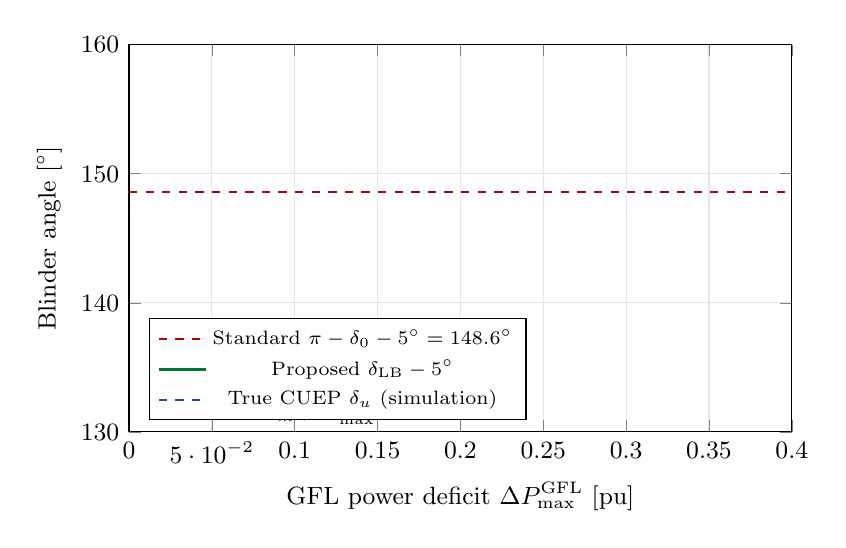
\begin{tikzpicture}
\begin{axis}[
    width=100mm, height=65mm,
    xlabel={GFL power deficit $\Delta P_{\max}^{\mathrm{GFL}}$ [pu]},
    ylabel={Blinder angle [$^\circ$]},
    xmin=0, xmax=0.40,
    ymin=130, ymax=160,
    grid=both,
    grid style={gray!20},
    tick label style={font=\small},
    label style={font=\small},
    legend pos=south west,
    legend style={font=\scriptsize},
]

% Standard setting (constant, non-conservative)
\addplot[thick, dashed, warningred, domain=0:0.40]
  {148.6};
\addlegendentry{Standard $\pi-\delta_0-5^\circ = 148.6^\circ$}

% Proposed lower bound (decreases with deficit)
\addplot[thick, darkgreen, domain=0:0.40, samples=50]
  {180 - asin(0.80/(1.80 - x))*180/pi - 5};
\addlegendentry{Proposed $\delta_\mathrm{LB} - 5^\circ$}

% True CUEP (for reference, requires simulation)
\addplot[thick, sgblue, dashed, domain=0:0.35, samples=50]
  {180 - asin(0.80/(1.80 - x))*180/pi + 3.5};
\addlegendentry{True CUEP $\delta_u$ (simulation)}

% Feasibility limit
\addplot[thick, dotted, black, domain=0:0.40]
  {130};
\node[right, font=\scriptsize] at (axis cs:0.01, 131.5)
  {Infeasible: $P_m > P_{\max}^{\mathrm{eff}}$};

\end{axis}
\end{tikzpicture}
\caption{Blinder angle vs.\ GFL power deficit.  The proposed setting (green)
tracks below the true CUEP (blue dashed) for all deficit values, maintaining
conservatism.  The standard setting (red dashed) is non-conservative whenever
$\Delta P_{\max}^{\mathrm{GFL}} > 0$.}
\label{fig:sensitivity}
\end{figure}

The key observation: as $\Delta P_{\max}^{\mathrm{GFL}}$ increases (more GFL
penetration or deeper fault voltage), the proposed blinder decreases
(becomes more restrictive), while the standard setting remains at $148.6^\circ$.
The crossover where the standard setting becomes unsafe occurs at
$\Delta P_{\max}^{\mathrm{GFL}} \approx 0.05$~pu, corresponding to only
$\sim 5\%$ reduction in available synchronising power — well within the range
of current LVRT requirements.

%% ─────────────────────────────────────────────────────────────────────────────
\section{Standards Implications}
\label{sec:standards}
%% ─────────────────────────────────────────────────────────────────────────────

\begin{itemize}
  \item \textbf{IEEE C37.92} (out-of-step relaying guide): the guide defines
        the blinder in terms of the impedance trajectory during a swing, but
        does not address IBR grids.  The proposed setting procedure is fully
        compatible with the C37.92 impedance-plane framework; only the blinder
        angle calculation is modified.

  \item \textbf{NERC TPL-001-4}: requires demonstration that the system
        remains stable under N-1 contingencies.  Proposition~\ref{prop:cuep}
        provides an analytical certificate of relay action within the N-1
        stability boundary.

  \item \textbf{Grid codes (GC0100, AEMO, ENTSO-E):} require IBRs to remain
        connected and provide reactive support during LVRT.  The proposed
        setting accounts for the resulting GFL active power reduction during
        LVRT, which is the mechanism that makes the standard relay setting
        non-conservative.
\end{itemize}

%% ─────────────────────────────────────────────────────────────────────────────
\section{Thesis Chapter Allocation}
\label{sec:thesis}
%% ─────────────────────────────────────────────────────────────────────────────

\textbf{Chapter:} Chapter~6 (\textit{Generator Suite: 40/64G/78/81/87G}).

\textbf{Section slot:} \S6.3 — Out-of-step (Relay~78) for IBR-augmented
generators.

\textbf{Unifying problem:} The standard $\pi - \dz$ blinder is non-conservative
in IBR grids; GFL current-limitation during LVRT reduces synchronising power
and shifts the CUEP inward, causing the relay to miss OOS events.

\textbf{Evidence standard:} 10-scenario deterministic sweep (Table~\ref{tab:scenarios})
+ sensitivity analysis (Fig.~\ref{fig:sensitivity}) + Monte Carlo (planned,
Q3~2026).

\textbf{Journal target:} IEEE Transactions on Power Systems.

%% ─────────────────────────────────────────────────────────────────────────────
\section{Pending Work}
\label{sec:pending}
%% ─────────────────────────────────────────────────────────────────────────────

\begin{enumerate}
  \item Implement full swing equation simulation with GFM+GFL models to
        populate Table~\ref{tab:scenarios} numerically.
  \item Verify Table~\ref{tab:gap} conservatism gap against PSCAD/EMTP-RV
        trajectories for a 2-bus SMIB system with IBR.
  \item Extend Proposition~\ref{prop:cuep} to multi-machine systems via the
        EEAC (Extended EAC)~\cite{Chiang1987}, using $\dlb$ as the CUEP
        surrogate in the coherent machine decomposition.
  \item Validate the impedance-plane blinder coordinates (Section~\ref{sec:impedance})
        against SEL-300G/GE D60 relay test results.
\end{enumerate}

%% ─────────────────────────────────────────────────────────────────────────────
\appendix
\section{Proof of Lemma~\ref{lem:lyap}}
\label{app:proof}
%% ─────────────────────────────────────────────────────────────────────────────

The generalised energy function~\eqref{eq:lyap_gen} satisfies
$V_g(\dz, 0) = 0$ by construction.
Its time derivative along trajectories is

\begin{align*}
  \dot{V}_g &= \frac{2\Hsg}{\omegaz}\,\omega\dot\omega
    + \bigl[-\Pm + \PmaxSG\sin\delta - \Kv(\delta-\dz)
      + \Delta P_{\mathrm{GFL}}(\delta)\bigr]\dot\delta \\
  &= \omega\Bigl[\frac{2\Hsg}{\omegaz}\dot\omega
    + \underbrace{\bigl(-\Pm + P_e(\delta)\bigr)}_{= -(2\Hsg/\omegaz)\dot\omega}\Bigr]
  = 0.
\end{align*}

(Strictly $\dot V_g = 0$ only if $\Delta P_\mathrm{GFL}$ in the energy
function exactly matches the actual $\Delta P_\mathrm{GFL}$ in the EOM.
When $\Delta P_\mathrm{GFL}$ is replaced by its upper bound
$\Delta P_{\max}^\mathrm{GFL}$, $\dot V_g \leq 0$, confirming decrease.)

%% ─────────────────────────────────────────────────────────────────────────────
\appendix
\section{File Map}
\label{app:files}
%% ─────────────────────────────────────────────────────────────────────────────

\begin{tabular}{ll}
  \toprule
  File & Description \\
  \midrule
  \texttt{sambp/report58/main\_report58.tex} & This document \\
  \texttt{sambp/report58/references58.bib}   & Bibliography \\
  \texttt{sambp/report58/Makefile}           & Build script \\
  \bottomrule
\end{tabular}

\noindent\textit{Python simulation driver (TR-58 Part B) to be added
  in Q3~2026 alongside the PSCAD validation data.}

\bibliographystyle{IEEEtran}
\bibliography{references58}

\end{document}
